\documentclass[tikz]{standalone}
\usepackage{tikz}
\usepackage{ifthen}

\begin{document}
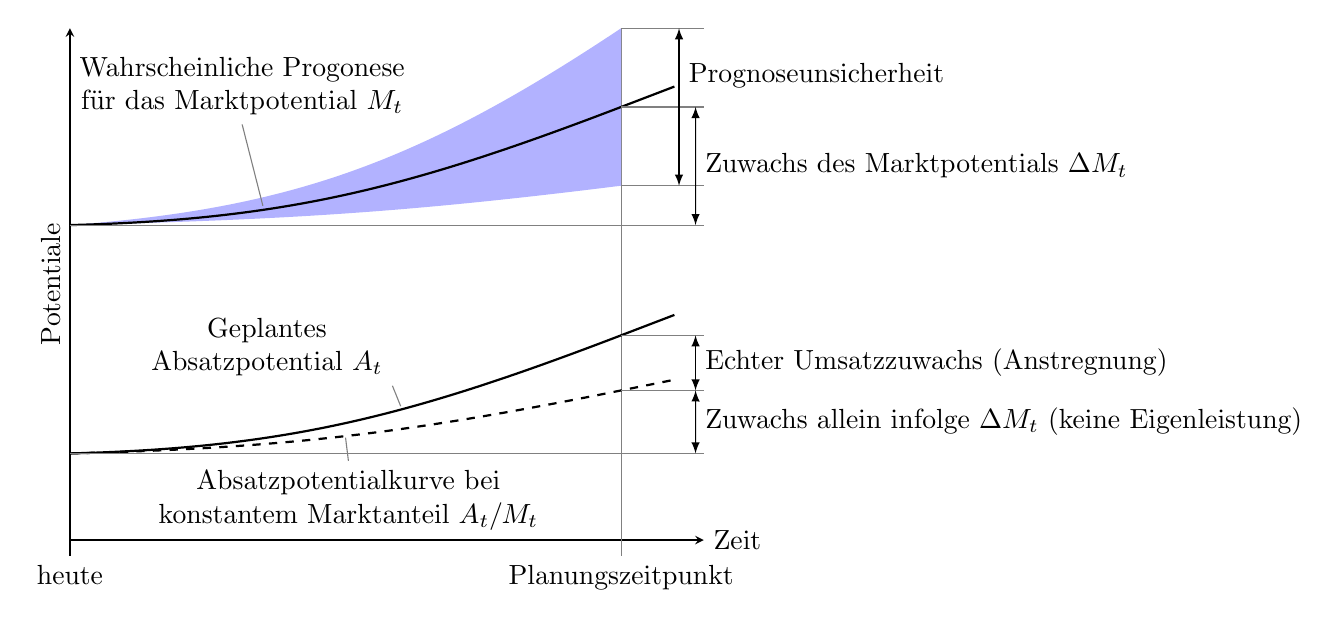
\begin{tikzpicture}[scale=1,
help lines/.style={gray},
xscale=.7,
arrow/.style={latex-latex}
]




\draw[-stealth] (0,0)--(11.5,0)node[right]{Zeit};
\draw[-stealth] (0,0)--(0,6.5)node[sloped, above, pos=.5]{Potentiale};
\draw(0,0)--++(0,-.2)node[below]{heute};
\draw[help lines] (10,-.2)node[below, black]{Planungszeitpunkt}--++(0,6.7);


\draw[thick, dashed] (0,1.1)coordinate(x)to[out=1, in = 188] ++(10,.8)coordinate(2)--++(8:1);
\path (x)--(2)coordinate[midway](2x);
\draw[help lines] (2x)++(0,-.2)--++(280:.3)node[below, align=center, black]{Absatzpotentialkurve bei \\ konstantem Marktanteil $A_t / M_t$};

\draw[thick] (x)to[out=1, in = 195] ++(10,1.5)coordinate(3)--++(15:1);
\path (x)--(3)coordinate[pos=.6](3x);
\draw[help lines] (3x)++(0,-.3)--++(120:.3)node[above left, align=center, black]{Geplantes \\ Absatzpotential $A_t$};

\draw[help lines] (x)--++(10,0)coordinate(1)--++(1.5,0)coordinate[pos=.9](1x);
\draw[help lines] (2)--++(1.5,0)coordinate[pos=.9](2x);
\draw[help lines] (3)--++(1.5,0)coordinate[pos=.9](3x);
\draw[arrow] (1x)--(2x) node[midway, right, align=left]{Zuwachs allein infolge $\Delta M_t$ (keine Eigenleistung)};
\draw[arrow] (2x)--(3x) node[midway, right, align=left]{Echter Umsatzzuwachs (Anstregnung)};






\fill[blue!30] (0,4)coordinate(x)to[out=1, in = 185] ++(10,.5)coordinate(2)--++(0,2)coordinate(4)to[out=205, in=3](x);
\draw[thick] (x)to[out=1, in = 195] ++(10,1.5)coordinate(3)--++(15:1);



\path (x)--(3)coordinate[pos=.35](3x);
\draw[help lines] (3x)++(0,-.28)--++(110:1.1)node[above, align=center, black]{Wahrscheinliche Progonese \\ für das Marktpotential $M_t$};
\draw[help lines] (x)--++(10,0)coordinate(1)--++(1.5,0)coordinate[pos=.9](1x);

\draw[help lines] (3)--++(1.5,0)coordinate[pos=.9](3x);
\draw[help lines] (2)--++(1.5,0)coordinate[pos=.7](2x);
\draw[help lines] (4)--++(1.5,0)coordinate[pos=.7](4x);


\draw[arrow] (1x)--(3x) node[midway, right, align=left]{Zuwachs des Marktpotentials $\Delta M_t$};
\draw[arrow] (2x)--(4x) node[pos=.7, right, align=left]{Prognoseunsicherheit};





\end{tikzpicture}
\end{document}